\newpage

\backgroundsetup{	scale=1,
				color=black,
				opacity=1,
				angle=0,
				contents={%
 						 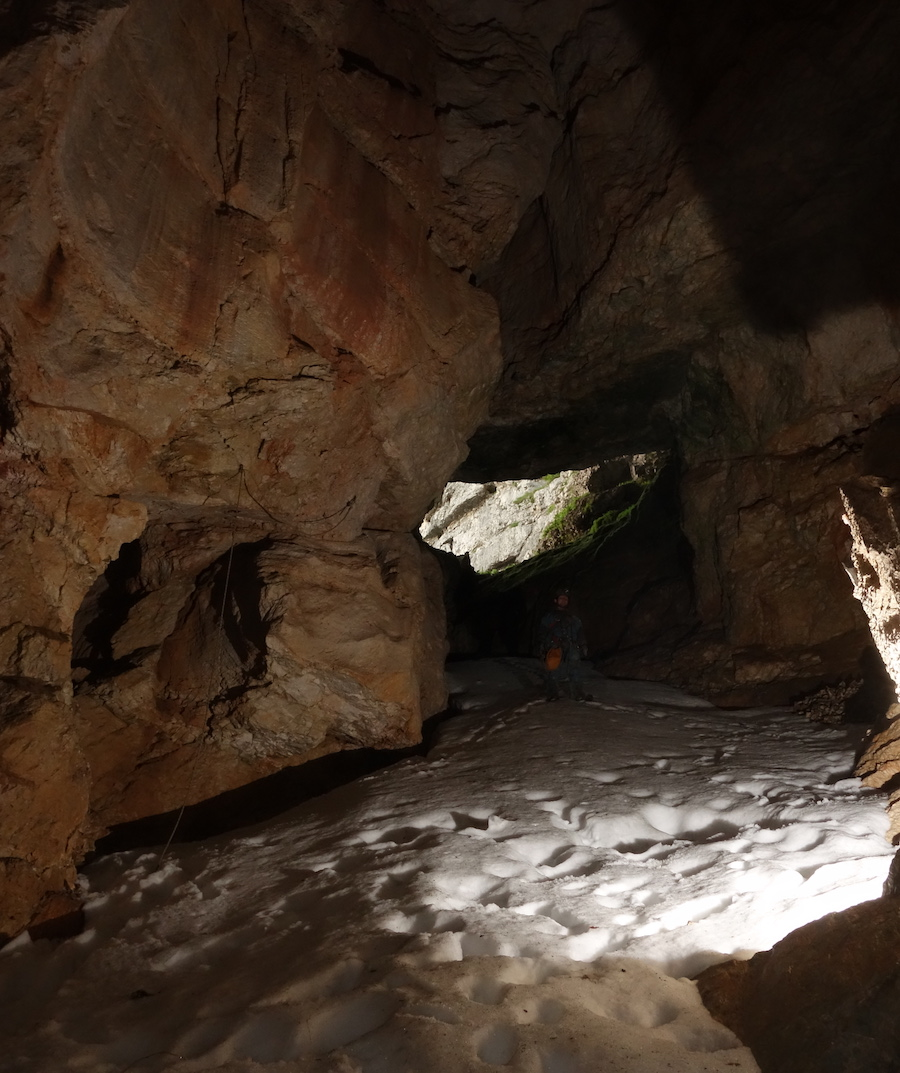
\includegraphics[height=\paperheight]{images/backgrounds/primadona-2016.jpg}
  				}
	}
\BgThispage

\begin{tcolorbox}
\chapter{2016 - Neprehojene Poti}
	\lettrine{T}{he} exploration target of the \emph{Neprehojene Poti} expedition to Slovenia was \passage{Primadona}, a 750\,m deep cave with an entrance imposingly 100\,m down the cliff on the Western side of the \passage{Migovec Plateau}. An impressive 2.6\,km long cave in its own right, it was connected in to the rest of \passage{Sistem Migovec} over the winter of 2015/2016 by our partner club the JSPDT. The connection point was between a high level passage in \passage{Monatip} and the southeastern end of \passage{NCB} passage. This means all the major cave systems on the plateau are now connected (until we find more).

	\passage{Primadona} had been explored sporadically over the preceding decade but mostly with the aim of going deep. The potential for leads relatively close to the surface (within 300\,m) was a major reason for going, in order to provide new cavers with a better shot at exploring new passages.

	The exploration was mainly focused in an area known as \passage{Rokovo Brezno} and over the course of the expedition was pushed 190\,m deeper and 835\,m further finally ending in a series of impressively large chambers.  A horizontal passage also connected with the other deep shaft series of \passage{Primadona}. Higher level leads also brought further 900\,m of passage, providing more links between \passage{Primadona} and \passage{Monatip} through \passage{Alkatraz} chamber.

	Unfortunately this year was not without incident and one of our party was injured whilst exploring 200\,m underground. Thanks to the exemplary reaction of all members of the expedition and heroic efforts of the Slovenian cave rescue service he was safely brought to the surface and is now fully recovered.
\end{tcolorbox}
